\documentclass{article}

\usepackage{arxiv}

\usepackage[utf8]{inputenc} % allow utf-8 input
\usepackage[T1]{fontenc}    % use 8-bit T1 fonts
\usepackage{lmodern}        % https://github.com/rstudio/rticles/issues/343
\usepackage{hyperref}       % hyperlinks
\usepackage{url}            % simple URL typesetting
\usepackage{booktabs}       % professional-quality tables
\usepackage{amsfonts}       % blackboard math symbols
\usepackage{nicefrac}       % compact symbols for 1/2, etc.
\usepackage{microtype}      % microtypography
\usepackage{graphicx}

\title{Neo Cocoon: Low-cost and Portable Neonatal Protection and
Development System}

\author{
    Karthik M Dani
   \\
    Dept of Medical Electronics Engineering \\
    B.M.S College of Engineering \\
  Bangalore - 560019 \\
  \texttt{\href{mailto:karthik.ml22@bmsce.ac.in}{\nolinkurl{karthik.ml22@bmsce.ac.in}}} \\
   \And
    Sanjana WG
   \\
    Dept of Medical Electronics Engineering \\
    B.M.S College of Engineering \\
  Bangalore - 560019 \\
  \texttt{\href{mailto:sanjana.ml22@bmsce.ac.in}{\nolinkurl{sanjana.ml22@bmsce.ac.in}}} \\
   \And
    Darshan S K
   \\
    Dept of Medical Electronics Engineering \\
    B.M.S College of Engineering \\
  Bangalore - 560019 \\
  \texttt{\href{mailto:darshan.ml22@bmsce.ac.in}{\nolinkurl{darshan.ml22@bmsce.ac.in}}} \\
  }


% tightlist command for lists without linebreak
\providecommand{\tightlist}{%
  \setlength{\itemsep}{0pt}\setlength{\parskip}{0pt}}


% Pandoc citation processing
%From Pandoc 3.1.8
% definitions for citeproc citations
\NewDocumentCommand\citeproctext{}{}
\NewDocumentCommand\citeproc{mm}{%
  \begingroup\def\citeproctext{#2}\cite{#1}\endgroup}
\makeatletter
 % allow citations to break across lines
 \let\@cite@ofmt\@firstofone
 % avoid brackets around text for \cite:
 \def\@biblabel#1{}
 \def\@cite#1#2{{#1\if@tempswa , #2\fi}}
\makeatother
\newlength{\cslhangindent}
\setlength{\cslhangindent}{1.5em}
\newlength{\csllabelwidth}
\setlength{\csllabelwidth}{3em}
\newenvironment{CSLReferences}[2] % #1 hanging-indent, #2 entry-spacing
 {\begin{list}{}{%
  \setlength{\itemindent}{0pt}
  \setlength{\leftmargin}{0pt}
  \setlength{\parsep}{0pt}
  % turn on hanging indent if param 1 is 1
  \ifodd #1
   \setlength{\leftmargin}{\cslhangindent}
   \setlength{\itemindent}{-1\cslhangindent}
  \fi
  % set entry spacing
  \setlength{\itemsep}{#2\baselineskip}}}
 {\end{list}}
\usepackage{calc}
\newcommand{\CSLBlock}[1]{#1\hfill\break}
\newcommand{\CSLLeftMargin}[1]{\parbox[t]{\csllabelwidth}{#1}}
\newcommand{\CSLRightInline}[1]{\parbox[t]{\linewidth - \csllabelwidth}{#1}\break}
\newcommand{\CSLIndent}[1]{\hspace{\cslhangindent}#1}

\begin{document}
\maketitle


\begin{abstract}
Enter the text of your abstract here.
\end{abstract}

\keywords{
    NICU
   \and
    Medical Device
   \and
    IoMT
   \and
    AI
   \and
    Neonatal Protection
   \and
    Portable
   \and
    Monitoring
   \and
    Premature Infants
   \and
    Temperature
   \and
    SpO2
   \and
    Heart Rate
   \and
    ECG
   \and
    Phototherapy
   \and
    Data Logging
   \and
    User-Friendly Interface
   \and
    Microprocessor
   \and
    Microcontroller
   \and
    Healthcare
   \and
    Jaundice Treatment
  }

\section{Introduction}\label{introduction}

Babies born before the completion of 37 weeks of pregnancy are
classified as premature {[}1{]}. They are further categorized as
follows:

\begin{enumerate}
\def\labelenumi{\arabic{enumi}.}
\item
  \textbf{Extremely premature:} Less than 28 weeks
\item
  \textbf{Very premature:} 28 to 32 weeks
\item
  \textbf{Moderate to late premature:} 32 to 37 weeks
\end{enumerate}

\subsection{Background}\label{background}

\subsubsection{Low Birth Weight (LBW) as consequence of Pre Mature
Birth}\label{low-birth-weight-lbw-as-consequence-of-pre-mature-birth}

\textbf{Low Birth Weight (LBW)} refers to infants born weighing less
than 5 pounds, 8 ounces (2,500 grams). In contrast, the average newborn
typically weighs around 8 pounds. Much of a baby's weight is accumulated
in the final weeks of pregnancy, so being born prematurely often results
in low birth weight {[}2{]}.

Another cause of Low Birth weight is condition called
\textbf{Intrauterine Growth Restriction (IUGR)} arises when a baby does
not grow adequately during pregnancy.

\paragraph{Health Complications of Low Birth
Weight}\label{health-complications-of-low-birth-weight}

Infants with low birth weight encounter numerous health complications
that can adversely affect their growth and development. One of the
significant issues they face is reduced oxygen levels at birth, which
may lead to immediate respiratory difficulties. These infants often
struggle to maintain a stable body temperature, putting them at risk for
hypothermia. Additionally, many experience feeding challenges, as their
ability to suck may be compromised, resulting in inadequate weight gain.
Their underdeveloped immune systems make them more susceptible to
infections. Furthermore, low birth weight can lead to breathing issues
like infant respiratory distress syndrome, stemming from immature lung
development. Neurological problems may also arise, such as
intraventricular hemorrhage, which involves bleeding within the brain.
The risk of digestive complications, particularly necrotizing
enterocolitis, poses further concerns. Lastly, there is an elevated risk
of sudden infant death syndrome (SIDS) during the early months of life,
adding to the vulnerabilities faced by these infants. {[}2{]}

\paragraph{3 methods to address Low Birth Weight as a Medical
Electronics
Engineer}\label{methods-to-address-low-birth-weight-as-a-medical-electronics-engineer}

Management for LBW often involves:

\begin{enumerate}
\def\labelenumi{\arabic{enumi}.}
\item
  Care in a neonatal intensive care unit (NICU).
\item
  Temperature-controlled environments such as a warmer or an infant
  incubator.
\item
  Specialized feeding methods, including tube feeding for infants unable
  to suck, or intravenous (IV) feeding.
\end{enumerate}

While we choose the 2nd method to address the problem, we choose
innovation in domain of incubators instead of warmers for the reasons
listed in the latter sections.

\section{Motivation}\label{motivation}

\subsection{Pre Mature Birth
Statistics}\label{pre-mature-birth-statistics}

In 2020, 10\% of all births worldwide, equating to approximately 13.4
million, were premature. In 2019, around 900,000 children died due to
complications arising from preterm birth. In low-income countries,
nearly half of the infants born at or before 32 weeks gestation (i.e.,
two months premature) do not survive due to a lack of effective and
affordable care {[}1{]} {[}3{]}. See figure \ref{fig:fig1}

Furthermore, more than 90\% of extremely preterm infants (born before 28
weeks) in low-income settings die within the first few days of life, in
stark contrast to less than 10\% in high-income countries. It is
estimated that three-quarters of these deaths could be averted with
existing, cost-effective interventions. The rate of premature births in
2020 varied from 4\% to 16\% {[}3{]}.

\begin{figure}
  \centering
  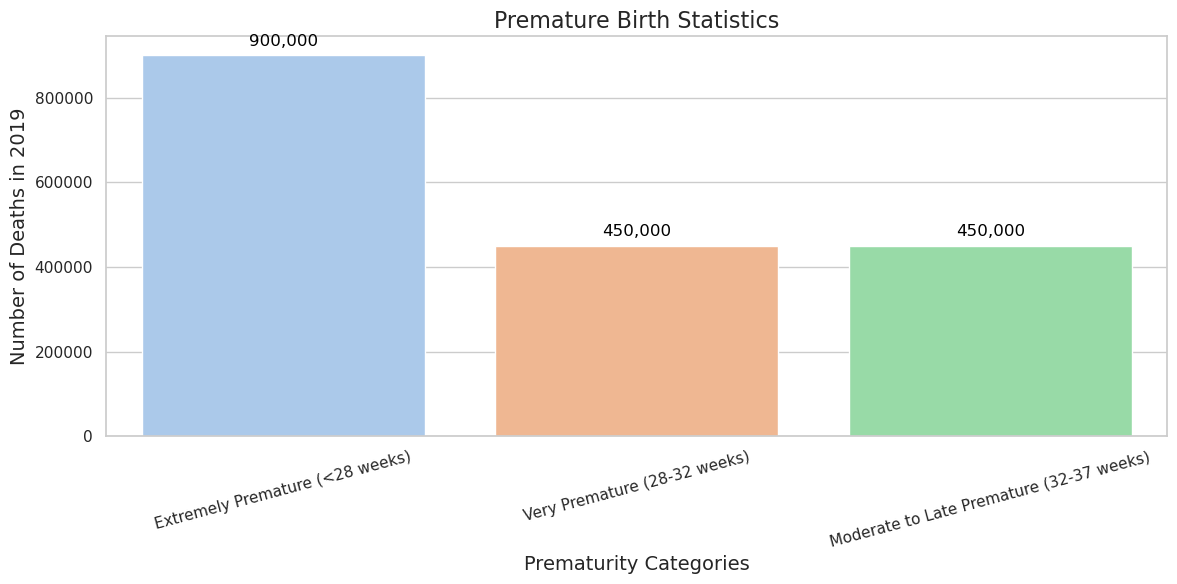
\includegraphics[width=350pt,height=200pt]{images/clipboard-1098342472.png} % Adjust the path to your image
  \caption{Sample figure caption.}
  \label{fig:fig1}
\end{figure}

In 2022, nearly half (47\%) of all deaths among children under five
years old took place during the neonatal period, which refers to the
first 28 days of life. Every day, approximately 6,500 newborns die,
primarily due to inadequate quality of care at birth. Most neonatal
deaths (about 75\%) occur within the first week of life, highlighting
the urgent need for effective interventions during this crucial
timeframe. {[}4{]} See figure \ref{fig:fig2}

\begin{figure}
  \centering
  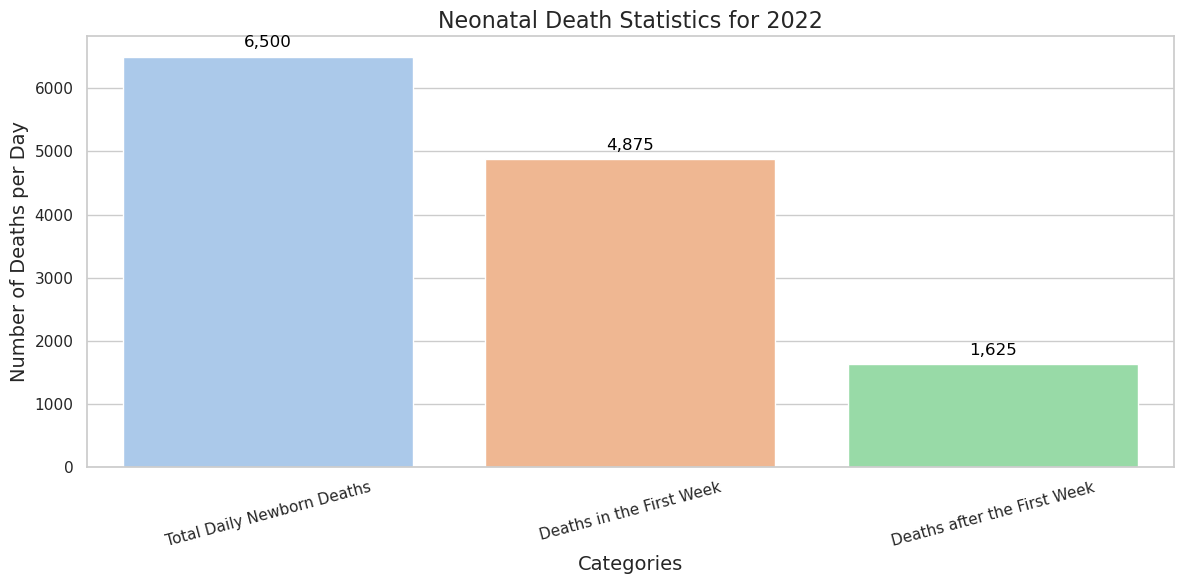
\includegraphics[width=350pt,height=200pt]{images/clipboard-3806704517.png} % Adjust the path to your image
  \caption{Sample figure caption.}
  \label{fig:fig2}
\end{figure}

Therefore the health outcomes for premature newborns in remote and
resource-limited areas stems from the critical need to address the
vulnerabilities these infants face. Premature babies are at a higher
risk of complications due to their underdeveloped physiological systems.
In regions where access to medical facilities and skilled healthcare
providers is limited, traditional neonatal care may not be feasible.
Thus, developing solutions that are smarter, safer, and responsive to
the unique challenges of these environments is essential. These
solutions should be designed to be user-friendly, minimizing the need
for extensive training and allowing caregivers to provide effective
support with limited resources. By focusing on reducing dependency on
human supervision, we can create reliable systems that ensure consistent
care for these vulnerable infants, ultimately aiming to improve their
survival rates and long-term health outcomes.

\section{Literature Survey}\label{literature-survey}

WHo claims Hypothermia is a significant contributor to neonatal illness
and death, particularly among low birth weight and normal newborns. To
combat this, thermal protection measures are crucial for maintaining a
normal body temperature of 36.5--37.5°C after birth, as newborns are
often exposed to cooler environments that cause rapid heat loss. {[}1{]}

\[
SizeOfInfant \propto T_{OutsideNormal}
\]

Where, \(T_{OutsideNormal}\) is the Temperature outside the normal
range.

This heat loss can occur through various mechanisms, including
evaporation, conduction, convection, and radiation, and can result in
significant temperature drops within the first 10-20 minutes
post-delivery. It's important to maintain a delivery room temperature
between 25--28°C, with a maximum tolerable temperature of around 35°C
for naked newborns. Separating newborns from their mothers complicates
thermal protection efforts and increases the risk of infections; thus,
immediate drying and wrapping of newborns are essential practices.
Hypothermia can be classified into three categories: mild (36--36.4°C),
moderate (32--35.9°C), and severe (\textless32°C), with prolonged
exposure leading to impaired growth and increased mortality rates. See
figure \ref{fig:fig3}

\begin{figure}
  \centering
  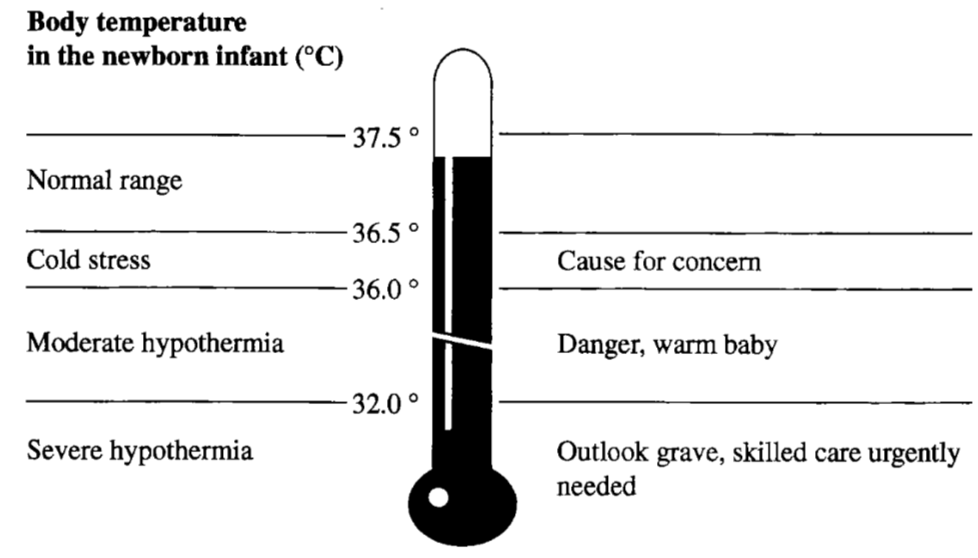
\includegraphics[width=350pt,height=200pt]{images/clipboard-2554530258.png} % Adjust the path to your image
  \caption{Sample figure caption.}
  \label{fig:fig3}
\end{figure}

Effective management includes assessing for infections and implementing
safe heating practices to avoid burns. Conversely, hyperthermia, defined
as a body temperature exceeding 37.5°C, can result in dehydration and
necessitates quick evaluation for infections. Guidelines for incubator
use specify maintaining an air temperature of 35--36°C, conducting
regular temperature checks, ensuring cleanliness, and encouraging
skin-to-skin contact between newborns and their mothers. {[}1{]}

The MQTT protocol has been evaluated in both the biomedical engineering
laboratory and the hospital's neonatology unit. Premature infants often
lack sufficient body fat and organ development to maintain their body
temperature, which should be kept between 28°C and 34°C. Reducing access
time to newborns is vital to minimize heat and oxygen loss. {[}5{]}

The BreathAnalyzer, a smartwatch that uses an AI model based on decision
trees, improves accuracy in detecting respiratory sinus arrhythmia (RSA)
from 35.37\% to 80\%, achieving an average of 42\% accuracy across
various scenarios. Calibration tests were conducted in accordance with
the ISO/IEC 1725:2017 standard to ensure measurement reliability.
Despite advancements, there are no existing devices that fully meet the
needs of the medical field. The Internet of Things in medicine (IoMT) is
essential for developing comprehensive technological solutions. However,
a progressive web application (SiMCa-Bio) was created to monitor
incubator conditions in real-time, focusing only on temperature,
humidity, and sound, with a sampling frequency of 5 minutes and data
transmission every 10 minutes {[}5{]}. Hoever Elevated levels of
relative humidity are not advisable for infants, as they can encourage
the growth of bacteria and germs {[}6{]}

The transition from traditional monitoring methods to wearable devices
focuses on reducing adhesive-related skin injuries. This approach
promotes the use of soft, flexible materials and gentler adhesion
techniques while emphasizing the design of all-in-one devices. The
priority is on non-invasive monitoring solutions that enhance
accessibility, particularly for high-risk patients, such as those born
prematurely (with a gestational age of less than 37 weeks) or with low
birth weight (typically less than 2.5 kg) {[}7{]}

Smart infant incubator monitoring and control system that utilizes a gas
sensor, accelerometer, and Peltier module, which are not part of our
current design was developed by K C N Raju {[}8{]}. The system
automatically adjusts the Peltier module and humidifier when
temperatures exceed 36°C to 37.2°C and humidity exceeds 60\%, ensuring
an optimal environment for premature and critically ill newborns.

A major challenge identified is the imbalance between caregivers and
patients, leading to increased workloads and compromised monitoring of
incubators. The study emphasizes maintaining temperatures between 36°C
and 37.5°C, with a targeted rectal temperature of around 36°C, and
humidity levels between 40\% and 60\%. Additionally, the integration of
artificial intelligence and live monitoring through cameras enhances the
care provided. However, limitations include the use of an Arduino Wi-Fi
R3 and reliance on an LCD display and ThingSpeak for IoT applications.

Another study {[}9{]} focuses on an IoT-based baby incubator monitoring
system utilizing Raspberry Pi Zero W. It monitors critical environmental
parameters, including temperature, humidity, and oxygen levels, in
real-time to safeguard infants in incubators. The system is connected to
a central computer for data visualization, alarms, and alerts, enabling
healthcare professionals to monitor the situation remotely. The
incubator is maintained at a temperature range of 32 to 36 degrees
Celsius to ensure the baby's skin remains at a healthy temperature of 37
degrees Celsius. Additionally, appropriate humidity levels warm the
baby's breath and facilitate the entry of moist air into the lungs.

Adding on to it, {[}10{]} emphasized that heating systems require
careful management, particularly during the winter months, to maintain a
consistent temperature for optimal comfort. Humidity levels in solids
and liquids are measured using hygrometers. Various methods for
measuring moisture include assessing changes in resistivity, variations
in capacitance, or monitoring the attenuation of microwaves.

This literature {[}10{]} provided information regarding checksum
{[}11{]} for a typical DHT22 sensor that was in communication via I2C
protocol:

\[ 
Data Structure = 8 bits (RH_{int}) + 8 bits (RH_{dec}) + 8 bits (T_{int}) + 8 bits (T_{dec}) + 8 Checksum Bits 
\]

Where, \(RH_{int}\) = Integer Relative Humidity, \(RH_{dec}\) = Decimal
Relative Humidity, \(T_{int}\) = Integer Temperature and \(T_{dec}\) =
Decimal Temperature

\section{Objectives}\label{objectives}

\subsection{Primary Objectives}\label{primary-objectives}

\begin{enumerate}
\def\labelenumi{\arabic{enumi}.}
\item
  \textbf{Affordablity}: Develop a low-cost yet cutting-edge device that
  enhances healthcare delivery in resource-limited settings, ensuring
  accessibility for all.
\item
  \textbf{Real-Time Monitoring of Essential Health Metrics}: Implement
  continuous monitoring capabilities for vital health parameters that
  includes body temperature, ambient temperature, ambient humidity
  levels, neonatal heart rate, blood oxygen saturation (\(SpO_2\)) and
  Electrocardiogram (ECG).
\item
  \textbf{User-Friendly Touch Screen Interface}: Design an intuitive
  touch-screen user interface that simplifies interaction with the
  device.
\item
  \textbf{Comprehensive Data Logging}: Facilitate automatic logging of
  health data over time, enabling caregivers to track trends and make
  informed decisions regarding the care of premature newborns.
\item
  \textbf{Remote Data Accessibility via IoT}: Enable remote access to
  device data through IoT integration, allowing healthcare professionals
  to monitor patients' conditions from distant locations, enhancing
  collaboration and response times.
\item
  \textbf{Critical Alarm System}: Integrate a robust alarm system that
  alerts caregivers to critical changes in health parameters, ensuring
  prompt action can be taken in emergencies.
\item
  \textbf{Phototherapy Capabilities}: Include a phototherapy function
  for the treatment of neonatal jaundice, utilizing advanced light
  therapy to support the health and recovery of affected infants.
\end{enumerate}

\subsection{Secondary Objectives}\label{secondary-objectives}

\begin{enumerate}
\def\labelenumi{\arabic{enumi}.}
\item
  \textbf{AI-Driven Jaundice Detection and Classification}: Explore the
  potential for AI integration to enhance jaundice detection and
  classification based on Kramer's rule. Availability of data is the
  major problem to implement this. A potential dataset {[}12{]} was
  found that can help us meet this objective.
\item
  \textbf{Produce Instantaneous Reports}: Create a reporting function
  that generates up-to-date health status reports, enabling healthcare
  professionals to swiftly evaluate the condition of premature infants
  without the need for manual data input.
\item
  \textbf{Compliance and Record Keeping}: Establish automated reporting
  that aligns with healthcare standards and regulations, simplifying the
  record-keeping process for neonatal care and ensuring accessibility
  for audits and assessments.
\end{enumerate}

\section{Materials and Methods}\label{materials-and-methods}

\subsection{Materials}\label{materials}

\subsubsection{Hardware requirements}\label{hardware-requirements}

\subsection{Footnotes}\label{footnotes}

Here is how you add footnotes. {[}\^{}Sample of the first footnote.{]}

\subsection{Tables}\label{tables}

See awesome Table\textasciitilde{}\ref{tab:table} which is written
directly in LaTeX in source Rmd file.

\begin{table}
 \caption{Sample table title}
  \centering
  \begin{tabular}{lll}
    \toprule
    \multicolumn{2}{c}{Part}                   \\
    \cmidrule(r){1-2}
    Name     & Description     & Size ($\mu$m) \\
    \midrule
    Dendrite & Input terminal  & $\sim$100     \\
    Axon     & Output terminal & $\sim$10      \\
    Soma     & Cell body       & up to $10^6$  \\
    \bottomrule
  \end{tabular}
  \label{tab:table}
\end{table}

\section*{References}\label{references}
\addcontentsline{toc}{section}{References}

\phantomsection\label{refs}
\begin{CSLReferences}{0}{0}
\bibitem[\citeproctext]{ref-noauthor_thermal_nodate}
\CSLLeftMargin{{[}1{]} }%
\CSLRightInline{{``Thermal protection of the newborn: A practical
guide.''} Accessed: Oct. 19, 2024. {[}Online{]}. Available:
\url{https://www.who.int/publications/i/item/WHO_RHT_MSM_97.2}}

\bibitem[\citeproctext]{ref-noauthor_low_nodate}
\CSLLeftMargin{{[}2{]} }%
\CSLRightInline{{``Low {Birth} {Weight}.''} Accessed: Oct. 19, 2024.
{[}Online{]}. Available:
\url{https://www.stanfordchildrens.org/en/topic/default?id=low-birth-weight-90-P02382}}

\bibitem[\citeproctext]{ref-noauthor_nacimientos_nodate}
\CSLLeftMargin{{[}3{]} }%
\CSLRightInline{{``Nacimientos prematuros.''} Accessed: Oct. 19, 2024.
{[}Online{]}. Available:
\url{https://www.who.int/es/news-room/fact-sheets/detail/preterm-birth}}

\bibitem[\citeproctext]{ref-noauthor_mortalidad_nodate}
\CSLLeftMargin{{[}4{]} }%
\CSLRightInline{{``Mortalidad neonatal.''} Accessed: Oct. 19, 2024.
{[}Online{]}. Available:
\url{https://www.who.int/es/news-room/fact-sheets/detail/newborn-mortality}}

\bibitem[\citeproctext]{ref-aya-parra_monitoring_2023}
\CSLLeftMargin{{[}5{]} }%
\CSLRightInline{P. A. Aya-Parra, A. J. Rodriguez-Orjuela, V. R. Torres,
N. P. C. Hernandez, N. M. Castellanos, and J. Sarmiento-Rojas,
{``Monitoring {System} for {Operating} {Variables} in {Incubators} in
the {Neonatology} {Service} of a {Highly} {Complex} {Hospital} through
the {Internet} of {Things} ({IoT}),''} \emph{Sensors (Basel,
Switzerland)}, vol. 23, no. 12, p. 5719, Jun. 2023, doi:
\href{https://doi.org/10.3390/s23125719}{10.3390/s23125719}.}

\bibitem[\citeproctext]{ref-pujiastuti_analysis_2022}
\CSLLeftMargin{{[}6{]} }%
\CSLRightInline{Y. Pujiastuti, A. Pudji, S. Y. Setiawan, F. Amrinsani,
and K. Phasinam, {``Analysis of {Temperature} {Stability} and {Accuracy}
on the {Design} of {Thermometer} {Calibrator} {Based} on {Fuzzy} {Logic}
{And} {On}/{Off} {Control},''} \emph{Journal of Electronics,
Electromedical Engineering, and Medical Informatics}, vol. 4, no. 3, pp.
144--153, Jul. 2022, doi:
\href{https://doi.org/10.35882/jeeemi.v4i3.244}{10.35882/jeeemi.v4i3.244}.}

\bibitem[\citeproctext]{ref-zhou_skin-interfacing_2024}
\CSLLeftMargin{{[}7{]} }%
\CSLRightInline{L. Zhou, M. Guess, K. R. Kim, and W.-H. Yeo,
{``Skin-interfacing wearable biosensors for smart health monitoring of
infants and neonates,''} \emph{Commun Mater}, vol. 5, no. 1, pp. 1--13,
May 2024, doi:
\href{https://doi.org/10.1038/s43246-024-00511-6}{10.1038/s43246-024-00511-6}.}

\bibitem[\citeproctext]{ref-k_c_n_smart_2024}
\CSLLeftMargin{{[}8{]} }%
\CSLRightInline{R. K C N, {``{SMART} {INFANT} {INCUBATOR} {MONITORING}
{AND} {CONTROL} {SYSTEM} {USING} {IoT},''} \emph{INTERNATIONAL JOURNAL
OF CREATIVE RESEARCH THOUGHTS}, vol. 12, pp. d786--d791, Mar. 2024.}

\bibitem[\citeproctext]{ref-ningsih_monitoring_2023}
\CSLLeftMargin{{[}9{]} }%
\CSLRightInline{F. Ningsih, B. Irianto, L. Lamidi, and M. Abdulhamid,
{``Monitoring {Baby} {Incubator} {Central} through {Internet} of
{Things} ({IoT}) based on {Raspberry} {Pi} {Zero} {W} with {Computer}
{Monitoring}),''} \emph{Indonesian Journal of Electronics,
Electromedical Engineering, and Medical Informatics}, vol. 5, pp.
116--124, Aug. 2023, doi:
\href{https://doi.org/10.35882/ijeeemi.v5i3.283}{10.35882/ijeeemi.v5i3.283}.}

\bibitem[\citeproctext]{ref-bogdan_sciendo_2016}
\CSLLeftMargin{{[}10{]} }%
\CSLRightInline{M. Bogdan, {``Sciendo,''} \emph{Acta Universitatis
Cibiniensis. Technical Series}, vol. 68, no. 1, pp. 22--25, Dec. 2016,
doi:
\href{https://doi.org/10.1515/aucts-2016-0005}{10.1515/aucts-2016-0005}.}

\bibitem[\citeproctext]{ref-maxino_effectiveness_2009}
\CSLLeftMargin{{[}11{]} }%
\CSLRightInline{T. C. Maxino and P. J. Koopman, {``The {Effectiveness}
of {Checksums} for {Embedded} {Control} {Networks},''} \emph{IEEE Trans.
Dependable and Secure Comput.}, vol. 6, no. 1, pp. 59--72, Jan. 2009,
doi:
\href{https://doi.org/10.1109/TDSC.2007.70216}{10.1109/TDSC.2007.70216}.}

\bibitem[\citeproctext]{ref-abdulrazzak_njn_2023}
\CSLLeftMargin{{[}12{]} }%
\CSLRightInline{A. Y. Abdulrazzak, S. L. Mohammed, and A. Al-Naji,
{``{NJN}: {A} {Dataset} for the {Normal} and {Jaundiced} {Newborns},''}
\emph{BioMedInformatics}, vol. 3, no. 3, pp. 543--552, Sep. 2023, doi:
\href{https://doi.org/10.3390/biomedinformatics3030037}{10.3390/biomedinformatics3030037}.}

\end{CSLReferences}

\bibliographystyle{unsrt}
\bibliography{/home/karthik/NeoCocoon/Synopsis/Neococoon Zotero Export
Literature/Neococoon Zotero Export Literature.bib}


\end{document}
